%!TEX root = ../template.tex
%%%%%%%%%%%%%%%%%%%%%%%%%%%%%%%%%%%%%%%%%%%%%%%%%%%%%%%%%%%%%%%%%%%%
%% chapter8.tex
%% NOVA thesis document file
%%
%% Chapter with the control architectures.
%%%%%%%%%%%%%%%%%%%%%%%%%%%%%%%%%%%%%%%%%%%%%%%%%%%%%%%%%%%%%%%%%%%%
\chapter{Control Architectures}
\label{cha:control_architectures}

\begin{quotation}
\begin{flushright}
\itshape
«Quotation»\\
\textbf{- Author}
\end{flushright}
\end{quotation}

This chapter will present the robotic control architectures used on the Panda robotic arm. Robot controllers are responsible for implementing an open/closed loop routine that controls each joint in order to move the robot to a specific position and keep it.

One main control architecture was used for robot autonomous movement. During co-manipulation a simplified architecture was used only to compensate gravity.

% ==========================
% = Overview =
% ==========================

\section{Overview}
\label{sec:control_architectures_overview}

For the particular application of this thesis, the robotic arm will generally move in free space while printing. Since the movement is in free space it makes sense to use a motion control strategy. However, because the task is executed close to the patient, there exists some probability of contact. When contact must be taken into consideration an interaction control strategy is more suited.\\

Since the control architecture must be able to manage robot motion along with interaction forces, a mathematical model is needed that relates them. The dynamic model of the robot provides that relation. On chapter \ref{cha:theoretical_concepts}, subsection \ref{subsec:dynamics}, it is shown that given a set of $n$ generalised coordinates $\boldsymbol{q} \in \mathbb{R}^n$ and a set of generalised torques $\boldsymbol{\tau} \in \mathbb{R}^n$
, the manipulator
dynamic model is

\begin{equation}
    \label{eq:robot_dynamic_model}
    \boldsymbol{M}(\boldsymbol{q})\ddot{\boldsymbol{q}} + \boldsymbol{C}(\boldsymbol{q}, \dot{\boldsymbol{q}})\dot{\boldsymbol{q}} + \boldsymbol{g}(\boldsymbol{q}) = \boldsymbol{\tau}.
\end{equation}

where $\boldsymbol{M}(\boldsymbol{q}) \in \mathbb{R}^{n\times n}$
is the inertia matrix, $\boldsymbol{C}(\boldsymbol{q}, \dot{\boldsymbol{q}})\dot{\boldsymbol{q}} \in \mathbb{R}^n$
is
the vector of Coriolis and centripetal terms and $\boldsymbol{g}(\boldsymbol{q}) \in \mathbb{R}^n$
is the gravity term.

% section control_architectures_overview

\section{Nonlinear Feedback Linearisation}
\label{sec:control_architectures_nonlinear_feedback_linearization}

The manipulator modelled by (\ref{eq:robot_dynamic_model}) is a nonlinear system. If the manipulator dynamic model is known \cite{Santos2018_computed_torque_control_robotic_assisted_tele_ecography}, a linear and decoupled
system can be achieved through nonlinear feedback linearisation. 
Let the total torques acting on the manipulator be given by

\begin{equation}
    \boldsymbol{\tau} = \boldsymbol{\tau}_c + \boldsymbol{\tau}_f + \boldsymbol{\tau}_m
\end{equation}

where $\boldsymbol{\tau}_c \in \mathbb{R}^n$, $\boldsymbol{\tau}_f \in \mathbb{R}^n$ and $\boldsymbol{\tau}_m \in \mathbb{R}^n$ are actuator, friction and interaction torques, respectively. By neglecting joint frictions
($\boldsymbol{\tau}_f \approx 0$) and defining $\boldsymbol{\tau}_m$ as the torque due to interaction

\begin{equation}
    \boldsymbol{\tau}_m = \boldsymbol{J}^T(\boldsymbol{q}) \boldsymbol{F}_m,
\end{equation}

the commanded torque $\boldsymbol{\tau}_c$ can be defined as

\begin{equation}
    \label{eq:tau_c}
    \boldsymbol{\tau}_c = \boldsymbol{C}(\boldsymbol{q}, \dot{\boldsymbol{q}})\dot{\boldsymbol{q}} + \boldsymbol{g}(\boldsymbol{q}) - \boldsymbol{\tau}_m +\boldsymbol{\tau}^\prime_c .
\end{equation}

$\boldsymbol{F}_m \in \mathbb{R}^m$ is a measurement of end-effector forces and $\boldsymbol{J}^T \in \mathbb{R}^{n\times m}$ is the Jacobian transpose.

From \ref{eq:tau_c} and \ref{eq:robot_dynamic_model}, the system reduces to

\begin{equation}
    \label{eq:tau_c_final}
    \boldsymbol{M}(\boldsymbol{q})\boldsymbol{\ddot{q}} = \boldsymbol{\tau}^\prime_c
\end{equation}

where $\boldsymbol{\tau}^\prime_c \in \mathbb{R}^n$ is the torque vector computed by the control law. When looking into task space, equation (\ref{eq:tau_c_final}) can be represented as \cite{Santos2018_computed_torque_control_robotic_assisted_tele_ecography}

\begin{equation}
    \label{eq:fp_lambdas}
    \boldsymbol{\Lambda}_p(\boldsymbol{q}) \boldsymbol{\ddot{x}}_p - \boldsymbol{\Lambda}_p(\boldsymbol{q}) \boldsymbol{\dot{J}}_p(\boldsymbol{q})\boldsymbol{\dot{q}} = \boldsymbol{F}_p    
\end{equation}

with

\begin{equation}
    \boldsymbol{\dot{x}}_p = \boldsymbol{J}_p(\boldsymbol{q})\boldsymbol{\dot{q}}
\end{equation}

\begin{equation}
    \boldsymbol{\ddot{x}}_p = \boldsymbol{J}_p(\boldsymbol{q})\boldsymbol{\ddot{q}} + \boldsymbol{\dot{J}}_p(\boldsymbol{q})\boldsymbol{\ddot{q}}
\end{equation}

\begin{equation}
    \boldsymbol{\Lambda}_p(\boldsymbol{q}) = (\boldsymbol{J}_p(\boldsymbol{q})\boldsymbol{M}^{-1}(\boldsymbol{q})\boldsymbol{J}^T_p(\boldsymbol{q}))^{-1}
\end{equation}

\begin{equation}
    \label{eq:tc_tp}
    \boldsymbol{\tau}^\prime_c = \boldsymbol{\tau}_p = \boldsymbol{J}^T_p(\boldsymbol{q})\boldsymbol{F}_p,
\end{equation}

where $\boldsymbol{\Lambda}_p(\boldsymbol{q}) \in \mathbb{R}^{m\times m}$ and $\boldsymbol{J}_p(\boldsymbol{q}) \in \mathbb{R}^{m\times n}$ are the inertia and Jacobian matrices associated with task $\boldsymbol{x}_p \in \mathbb{R}^m$. $\boldsymbol{\tau}_p \in \mathbb{R}^n$ and $\boldsymbol{F}_p \in \mathbb{R}^m$ are respectively, torque and force vectors computed by the controller to perform $\boldsymbol{x}_p$.

% section control_architectures_nonlinear_feedback_linearization

\section{Null-Space Control}
\label{sec:control_architectures_nullspace_control}

When a robotic system is task redundant, the number of degrees of freedom of the task, $m$, is less than the degrees of freedom of the robot, $n$. In this case, the robot can accomplish a designated task with several different joint configurations. It is operating in the null-space of the primary controller, which is the region of the state space where there is a redundancy of solutions.

In these situations, it is possible to create another controller dedicated to accomplishing a secondary task, operating in the null-space of the primary controller. The full control signal will be the combination of the primary signal and a filtered version of the secondary signal. Filtering the secondary signal means that the secondary goals can only be accomplished if they do not affect the performance of the primary controller.\\

Mathematically, if $m < n$, the system is redundant when performing $\boldsymbol{x}_p$ and $\boldsymbol{\tau}^\prime_c$ is not unique \cite{Santos2018_computed_torque_control_robotic_assisted_tele_ecography}. The generalised torque/force relationship is given by

\begin{equation}
    \label{eq:null_space_tau_prime_c}
    \boldsymbol{\tau}^\prime_c = \boldsymbol{J}^T_p(q) \boldsymbol{F}_p + \boldsymbol{N}^T_p(q) \boldsymbol{\tau}_s.
\end{equation}

This relationship allows the decomposition of $\boldsymbol{\tau}^\prime_c$ into two
dynamically decoupled torque vectors 

\begin{equation}
    \boldsymbol{\tau}^\prime_c = \boldsymbol{\tau}_p + \boldsymbol{\tau}_n,
\end{equation}

being $\boldsymbol{\tau}_p$ the torque performing the primary task (see (\ref{eq:tc_tp})) and

\begin{equation}
    \boldsymbol{\tau}_n = \boldsymbol{N}^T_p(\boldsymbol{q}) \boldsymbol{\tau}_s
\end{equation}

the torque of a secondary task that does not interfere with $\boldsymbol{\tau}_p$ and is performed in the null-space of $\boldsymbol{J}^T_p (\boldsymbol{q})$. $\boldsymbol{N}^T_p(\boldsymbol{q})$ is given by 

\begin{equation}
    \boldsymbol{N}^T_p(\boldsymbol{q}) = [\boldsymbol{I} - ¯\boldsymbol{\bar{J}}_p(\boldsymbol{q}) \boldsymbol{J}_p(\boldsymbol{q})]^T = [\boldsymbol{I} - \boldsymbol{J}^T_p(\boldsymbol{q}) ¯\boldsymbol{\bar{J}}^T_p(\boldsymbol{q})],
\end{equation}

where $\boldsymbol{N}^T_p(\boldsymbol{q}) \in \mathbb{R}^{n\times n}$ is the null-space projector of $\boldsymbol{x}_p, \boldsymbol{I} \in \mathbb{R}^{n\times n}$ the identity matrix and $\boldsymbol{\bar{J}}_p(\boldsymbol{q}) \in \mathbb{R}^{m\times n}$ is the dynamically
consistent generalized inverse of $\boldsymbol{J}_p(\boldsymbol{q})$ \cite{Santos2018_computed_torque_control_robotic_assisted_tele_ecography}, given by 

\begin{equation}
    \boldsymbol{\bar{J}}p(\boldsymbol{q}) = \boldsymbol{M}^{-1}(\boldsymbol{q}) \boldsymbol{J}^T_p(\boldsymbol{q}) \boldsymbol{\Lambda}_p(\boldsymbol{q}).
\end{equation}

% section control_architectures_nullspace_control

\section{Impedance Control}
\label{sec:control_architectures_impedance_control}

There are various interaction control architectures. The one chosen for the task was impedance control. The concept behind this architecture is to model the robot-environment interaction dynamics as mass-spring-damper system dynamics \cite{Ott2008_cartesian_impedance_control}. Figures \ref{fig:impedance_control_robot_environment_model} and \ref{fig:impedance_control_robot_environment_force} show a representation of robot-environment interaction using this model.

\begin{figure*}[htbp]
	\begin{minipage}[b]{.48\textwidth}
	\centering
	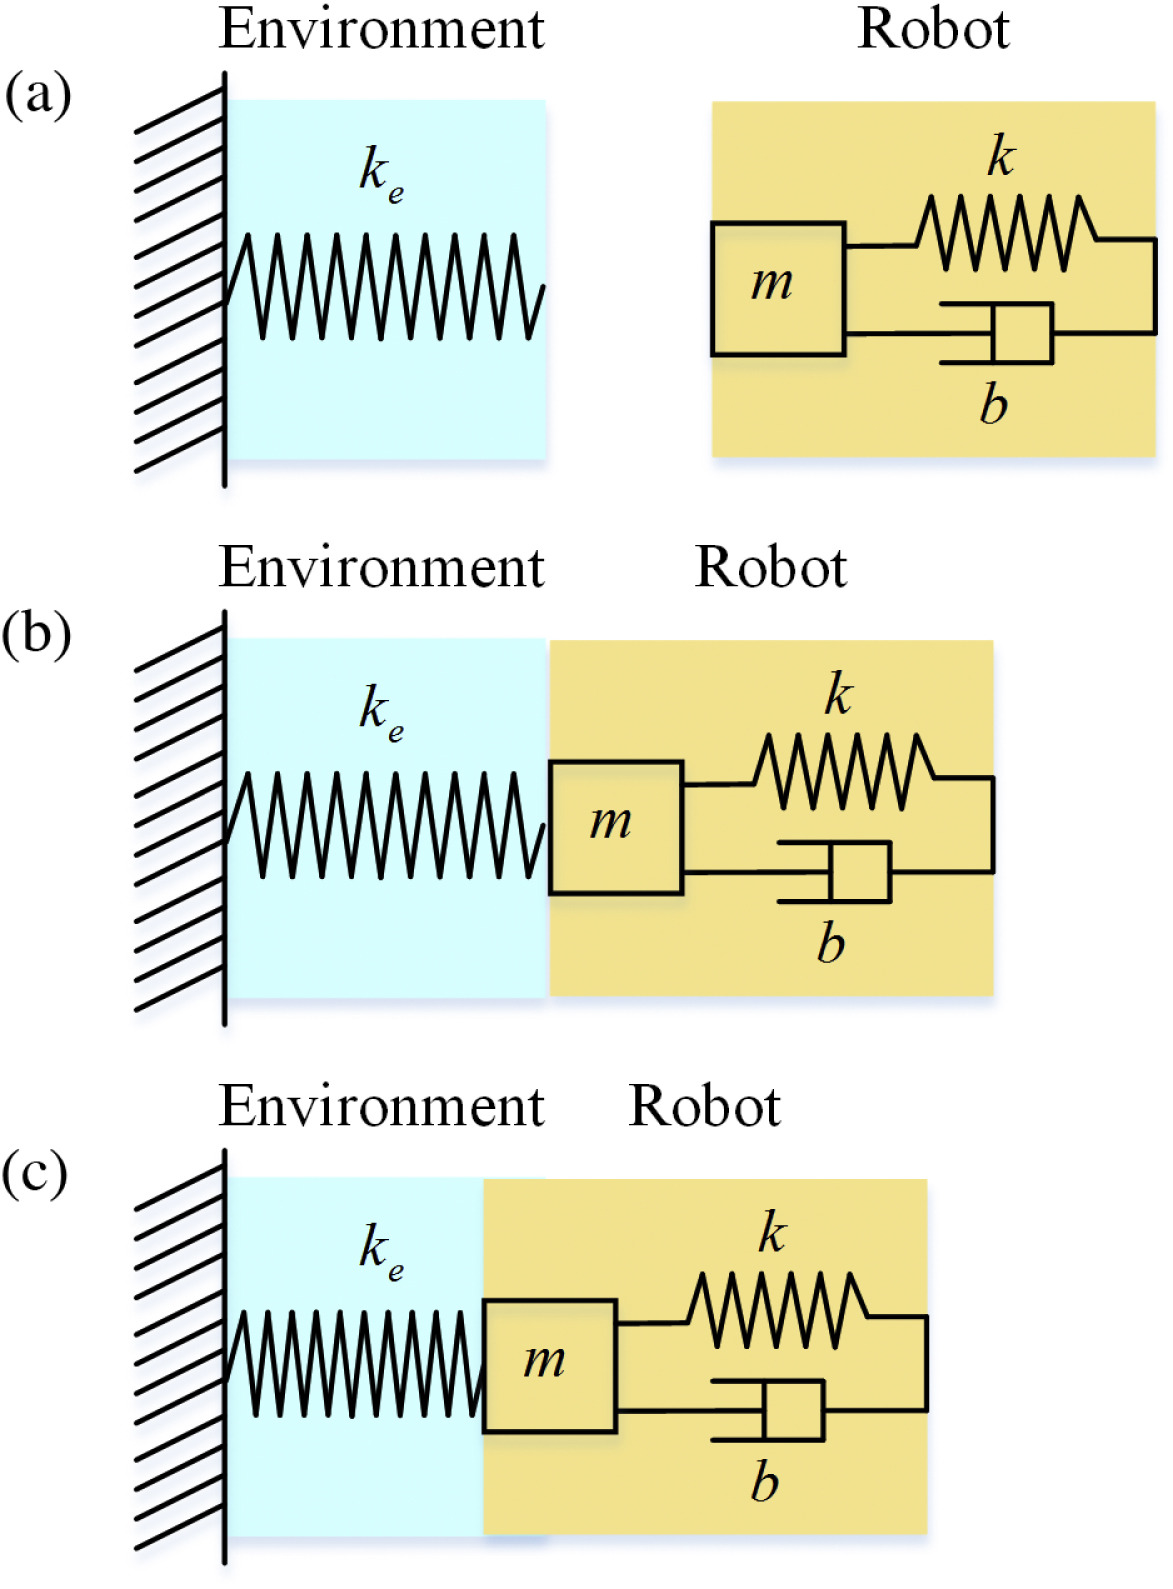
\includegraphics[width=\linewidth]{impedance_control_robot_environment_model}
	\caption{System model of robot and rigid environment: (a) without any contact between robot and environment, (b) critical point when contact occurs but $f = 0$ and (c) contact with $f \neq 0$. \cite{Duan2018_adaptive_variable_impedance_control}}
	\label{fig:impedance_control_robot_environment_model}
	\end{minipage}%
	\hfill
	\begin{minipage}[b]{.48\textwidth}
	\centering
	\raisebox{1.1in}{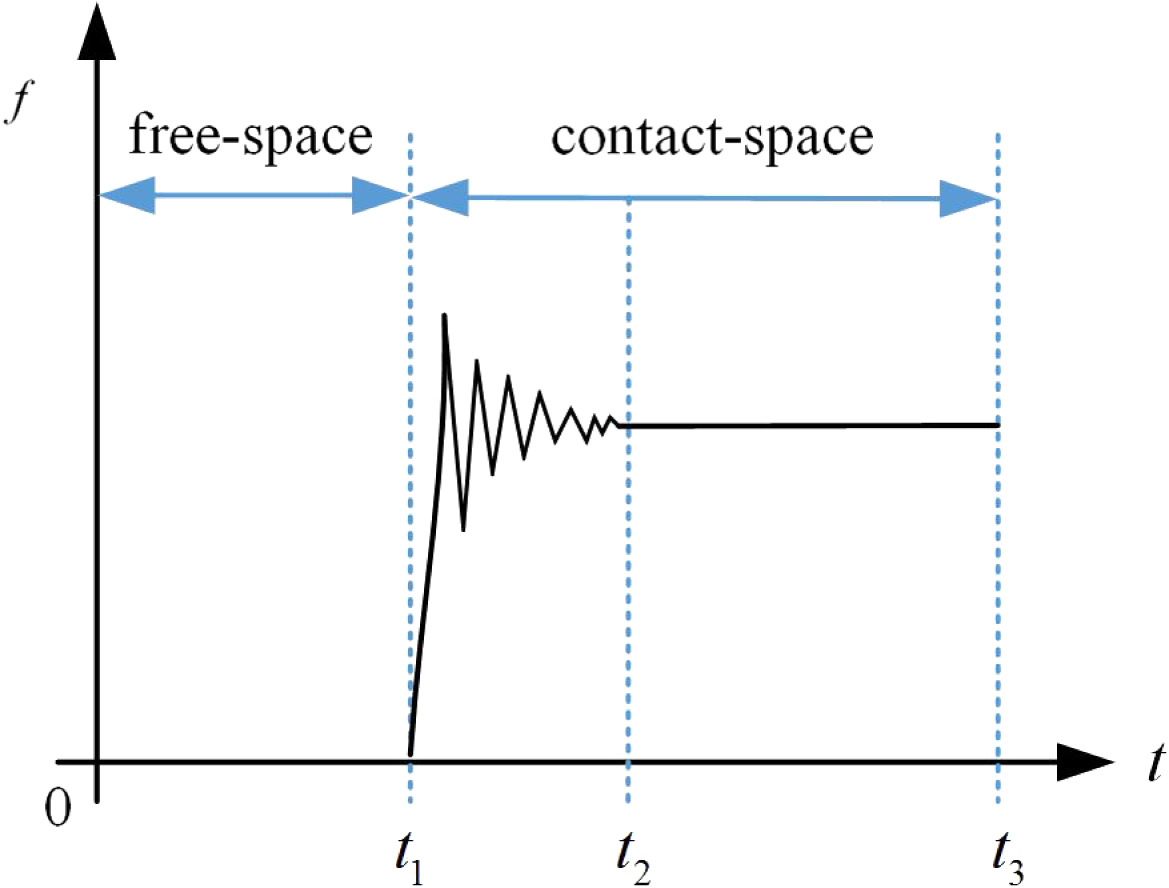
\includegraphics[width=\linewidth]{impedance_control_robot_environment_force}}
	\caption{The diagram of robot and environment contact force. \cite{Duan2018_adaptive_variable_impedance_control}}
	\label{fig:impedance_control_robot_environment_force}
	\end{minipage}
\end{figure*}

On this model, the end-effector velocity $\dot{X}$ and the robot applied force $F_e$ are related to a mechanical impedance $Z$. In the Laplace domain,

\begin{equation}
    \label{eq:impedance_and_force}
    -F_e(s) = Z(s) \dot{X}(s)
\end{equation}

with

\begin{equation}
    \label{eq:impedance_model}
    sZ(s) = As^2 + Ds + K
\end{equation}

where A, K and D are the parameters of a mass-spring-damper system, respectively.

If the analysis is done in the time domain, for an equilibrium point $\boldsymbol{x}_p$, the external force $\boldsymbol{F}_e$ is given by

\begin{equation}
    \label{eq:impedance_time_domain}
    \boldsymbol{A}(\boldsymbol{\ddot{x}}_p - \boldsymbol{\ddot{x}}_d)+\boldsymbol{D}(\boldsymbol{\dot{x}}_p - \boldsymbol{\dot{x}}_d) + \boldsymbol{K}(\boldsymbol{x}_p - \boldsymbol{x}_d) = \boldsymbol{F}_e.
\end{equation}

In the task space, the force $\boldsymbol{F}_p$ (see (\ref{eq:tc_tp})) is actually the sum of commanded force $\boldsymbol{F}_c$ with the environment force $\boldsymbol{F}_e$, made by external forces applied to the robot body, 

\begin{equation}
    \boldsymbol{F}_p = \boldsymbol{F}_c + \boldsymbol{F}_e.
\end{equation}

Making 

\begin{equation}
    \boldsymbol{F}_c = -\boldsymbol{\Lambda}_p(\boldsymbol{q}) \boldsymbol{\dot{J}}_p(\boldsymbol{q}) \boldsymbol{\dot{q}} + \boldsymbol{F}^*_p ,
\end{equation}

and knowing from (\ref{eq:fp_lambdas}), 

\begin{equation}
    \boldsymbol{\Lambda}_p(\boldsymbol{q}) \boldsymbol{\ddot{x}}_p = \boldsymbol{F}^*_p + \boldsymbol{F}_e,
\end{equation}

where $\boldsymbol{F}^*_p$ is a new control variable. Assigning to $\boldsymbol{F}^*_p$ the following control law 

\begin{equation}
    \label{eq:Fp_lambda_ADK}
    \boldsymbol{F}^*_p = \boldsymbol{\Lambda}_p(\boldsymbol{q}) \boldsymbol{\ddot{x}}_p - [\boldsymbol{A}(\boldsymbol{\ddot{x}}_p - \boldsymbol{\ddot{x}}_d) + \boldsymbol{D}(\boldsymbol{\dot{x}}_p - \boldsymbol{\dot{x}}_d) + \boldsymbol{K}(\boldsymbol{x}_p  -\boldsymbol{x}_d)].
\end{equation}

In practice, inertia shaping is hard to implement since $\boldsymbol{\ddot{x}}_p$ is too noisy, so the mass term $\boldsymbol{A}$ is considered

\begin{equation}
    \boldsymbol{A} = \boldsymbol{\Lambda}_p(\boldsymbol{q}) = (\boldsymbol{J}_p(\boldsymbol{q}) \boldsymbol{M}^{-1}(\boldsymbol{q}) \boldsymbol{J}^T_p (\boldsymbol{q}))^{-1}.
\end{equation}

Therefore, (\ref{eq:Fp_lambda_ADK}) can be rewritten by

\begin{equation}
    \label{eq:Fp_lambda_ADK_simplified}
    \boldsymbol{F}^*_p = \boldsymbol{\Lambda}_p(\boldsymbol{q}) \boldsymbol{\ddot{x}}_d + \boldsymbol{D} (\boldsymbol{\dot{x}}_d - \boldsymbol{\dot{x}}_p) + \boldsymbol{K} (\boldsymbol{x}_d - \boldsymbol{x}_p).
\end{equation}

From (\ref{eq:Fp_lambda_ADK_simplified}), (\ref{eq:tc_tp}) is now given by

\begin{equation}
    \label{eq:tau_p_final}
    \boldsymbol{\tau}_p = \boldsymbol{J}^T_p(\boldsymbol{q}) \boldsymbol{F}_p = \boldsymbol{J}^T_p (-\boldsymbol{\Lambda}_p(\boldsymbol{q}) \boldsymbol{\dot{J}}_p(\boldsymbol{q}) \boldsymbol{\dot{q}} + \boldsymbol{F}^*_p).
\end{equation}

Since the derivative Jacobian $\boldsymbol{\dot{J}}_p(\boldsymbol{q})$ has a small influence on the system it is ignored over this work, which results in a simplification of (\ref{eq:tau_p_final}),

\begin{equation}
    \boldsymbol{\tau}_p = \boldsymbol{J}^T_p \boldsymbol{F}^*_p .
\end{equation}

% section control_architectures_impedance_control

\section{Posture Optimisation}
\label{sec:control_architectures_posture_optimisation}

Besides guaranteeing that the robot executes its task with efficacy, efficiency is also desirable. For efficiency, the robot performance must be optimised. The manipulator posture plays a key role in performance optimization \cite{Ochoa2019_control_architecture_robotic_polishing}. 

When the joints are close to their limits, oftentimes problems with singularities arise. To avoid such problems, a secondary task is created to keep the robot redundant joints close to the middle of their range value through gradient minimisation \cite{Santos2018_computed_torque_control_robotic_assisted_tele_ecography}.

This is obtained by projecting $\boldsymbol{\tau}_s$ in the null-space of the main task (see (\ref{eq:null_space_tau_prime_c}))

\begin{equation}
    \boldsymbol{\tau}_s = \boldsymbol{M}(\boldsymbol{q}) \boldsymbol{K}_N \frac{\partial\boldsymbol{\nu}(\boldsymbol{q})}{\partial\boldsymbol{q}},
\end{equation}

where $\boldsymbol{K}_N \in \mathbb{R}^{n\times n}$ is a diagonal gain matrix and $\boldsymbol{\nu}(\boldsymbol{q})$ is an objective function given by

\begin{equation}
    \boldsymbol{\nu}(\boldsymbol{q}) = - \frac{1}{2} \sum_{i=1}^{n}  \left(\frac{\boldsymbol{q}_i - \boldsymbol{\bar{q}}_i}{\boldsymbol{q}_{iM} - \boldsymbol{q}_{im}}\right)^2,
\end{equation}

where $\boldsymbol{\bar{q}}_i$, $\boldsymbol{q}_{iM}$ and $\boldsymbol{q}_{im}$ are, respectively, the ith joint middle, maximum and minimum range value.

% section control_architectures_posture_optimisation

\section{Cartesian Impedance Controller with Posture Optimisation}
\label{sec:control_architectures_cartesian_impedance_posture_optimisation}

In this section, the controller will be described. It will start with the position control, then goes on to orientation control, and ends with the architecture.

The task force $\boldsymbol{F^*_p}$ is a concatenation of a 3D force vector $\boldsymbol{f}$ and a 3D torque vector $\boldsymbol{\mu}$ \cite{Ochoa2019_control_architecture_robotic_polishing}:

\begin{equation}
    \label{eq:task_force_matrix_notation}
    \boldsymbol{F^*_p} = \begin{bmatrix}
    \boldsymbol{f}\\
    \boldsymbol{\mu}
    \end{bmatrix}.
\end{equation}

\subsection{Position Controller}
\label{subsec:control_architectures_cartesian_impedance_posture_optimisation_position_controller}

According to \citeauthor{Ochoa2019_control_architecture_robotic_polishing} \cite{Ochoa2019_control_architecture_robotic_polishing}, if $\boldsymbol{p}_c$ and $\boldsymbol{p}_d$ are respectively the current and desired end-effector positions, and considering $\ddot{\boldsymbol{p}}_d$ and $\dot{\boldsymbol{p}}_d$ as null vectors, the 3D force vector $\boldsymbol{f}$ is computed by (\ref{eq:position_controller_force}).

\begin{equation}
    \label{eq:position_controller_force}
    \boldsymbol{f} = -\boldsymbol{D}_p \dot{\boldsymbol{p}}_c + \boldsymbol{K}_p \Delta \boldsymbol{p}_{cd} + \boldsymbol{I}_p \boldsymbol{i}_{ep}.
\end{equation}

$\Delta \boldsymbol{p}_{cd}$ is the position error (\ref{eq:position_controller_error}) and $\boldsymbol{i}_{ep}$ represents the position integral error (\ref{eq:position_controller_integral_error}).

$\boldsymbol{D}_p \in R^{3\times3}$, $\boldsymbol{K}_p \in R^{3\times3}$ and $\boldsymbol{I}_p \in R^{3\times3}$ are diagonal gain matrices referred to position damping, stiffness and integral gains, respectively. In (\ref{eq:position_controller_error}) and (\ref{eq:position_controller_integral_error}) $k$ is the iteration number in a real-time control loop at 1 kHz frequency.

\begin{equation}
    \label{eq:position_controller_error}
    \Delta \boldsymbol{p}_{cd}[k] = \boldsymbol{p}_d[k] - \boldsymbol{p}_c[k].
\end{equation}

\begin{equation}
    \label{eq:position_controller_integral_error}
    \boldsymbol{i}_{ep}[k] = \boldsymbol{i}_{ep}[k-1] + \Delta \boldsymbol{p}_{cd}[k],
\end{equation}

% subsection control_architectures_cartesian_impedance_posture_optimisation_position_controller

\subsection{Orientation Controller}
\label{subsec:control_architectures_cartesian_impedance_posture_optimisation_orientation_controller}

As with the position controller, on the orientation controller the error must also be considered on the impedance model.

The orientation error is a bit more complex to calculate so additional formulation is required. The computation of the rotation error from the current to the desired orientation, described in the base frame, $R_{c\to d}$, is given by \cite{Ochoa2019_control_architecture_robotic_polishing}

\begin{equation}
    \label{eq:orientation_controller_error}
    \boldsymbol{R}_{c\to d} = \boldsymbol{R}_d \boldsymbol{R}^{-1}_c,
\end{equation}

where $\boldsymbol{R}_c$ is the current end-effector orientation and $\boldsymbol{R}_d$ the desired one. Instead of using directly rotation matrices, a simpler representation derived from the Angle-Axis format was used \cite{Ochoa2019_control_architecture_robotic_polishing}. Given the rotation matrix $\boldsymbol{R}$ represented by

\begin{equation}
    \label{eq:orientation_controller_rotation_matrix}
    \boldsymbol{R} = \begin{bmatrix} 
    r_{11} & r_{12} & r_{13}\\
    r_{21} & r_{22} & r_{23}\\
    r_{31} & r_{32} & r_{33}
    \end{bmatrix},
\end{equation}

the associated Angle-Axis representation is

\begin{equation}
    \label{eq:orientation_controller_angle_axis}
    \begin{cases}
        \theta = \cos^{-1}\left({\frac{r_{11}+r_{22}+r_{33}-1}{2}} \right)\\
        \boldsymbol{\nu} = \frac{1}{2\sin{\theta}} \begin{bmatrix}
        r_{32} - r_{23}\\
        r_{13} - r_{31}\\
        r_{21} - r_{12}
        \end{bmatrix}
    \end{cases},
\end{equation}

where $\theta$ is the angle and $\boldsymbol{\nu}$ is an unitary vector. From $\boldsymbol{\nu}$, a rotation vector $\boldsymbol{r}$ that has no singularity issues or fraction computations can be obtained through (\ref{eq:orientation_controller_rotation_vector}).

\begin{equation}
    \label{eq:orientation_controller_rotation_vector}
    \boldsymbol{r} = \boldsymbol{\nu} \sin{\theta} = \frac{1}{2} \begin{bmatrix}
        r_{32} - r_{23}\\
        r_{13} - r_{31}\\
        r_{21} - r_{12}
        \end{bmatrix}
\end{equation}

The transformation of a rotation matrix into a rotation vector (\ref{eq:orientation_controller_rotation_vector}) is represented by the function $R2r(\cdot)$ like

\begin{equation}
    \boldsymbol{r} = R2r(\boldsymbol{R})
\end{equation}

Applying $R2r(\cdot)$ to $\boldsymbol{R}_{c\to d}$ a rotation vector $\boldsymbol{r}_{c\to d}$ is obtained,
which represents the orientation error $\Delta \boldsymbol{o}_{cd}$, in base coordinates.

\begin{equation}
    \Delta \boldsymbol{o}_{cd} \equiv \boldsymbol{r}_{c\to d} = R2r(\boldsymbol{R}_{c\to d}). 
\end{equation}

Therefore, considering null vectors the desired angular
velocity ($\boldsymbol{w}_d$) and acceleration ($\boldsymbol{\alpha}_d$), the 3D torque vector $\boldsymbol{\mu}$ is computed by

\begin{equation}
    \boldsymbol{\mu} = -\boldsymbol{D}_o w_c + \boldsymbol{K}_o \Delta \boldsymbol{o}_{cd} + \boldsymbol{I}_o \boldsymbol{i}_{eo},
\end{equation}

where $\boldsymbol{D}_o \in \mathbb{R}^{3\times3}$, $\boldsymbol{K}_o \in \mathbb{R}^{3\times3}$ and $\boldsymbol{I}_o \in \mathbb{R}^{3\times3}$ are diagonal gain matrices referred to orientation damping, stiffness and integral gains, respectively. $\boldsymbol{i}_{eo}$ represents the orientation integral error. It is computed by iteratively projecting and adding the previous error vector $\Delta \boldsymbol{o}_{cd}[k-1]$ to the current error vector $\Delta \boldsymbol{o}_{cd}[k]$. The calculation depends on the error vector squared. For $\delta \ll 1$,

\begin{itemize}
    \item if $(\Delta \boldsymbol{o}_{cd}[k])^T \Delta \boldsymbol{o}_{cd}[k] < \delta$:
        \begin{equation}
            \boldsymbol{i}_{eo}[k] = \Delta \boldsymbol{o}_{cd}[k]
        \end{equation}
        
    \item else:
        \begin{equation}
            \boldsymbol{i}_{eo}[k] = \left[ \left( (\boldsymbol{i}_{eo}[k-1])^T \frac{\Delta \boldsymbol{o}_{cd}[k]}{\| \Delta \boldsymbol{o}_{cd}[k] \|} \right) \frac{\Delta \boldsymbol{o}_{cd}[k]}{\| \Delta \boldsymbol{o}_{cd}[k] \|} \right] + \boldsymbol{o}_{cd}[k]
        \end{equation}
\end{itemize}

The current linear and angular velocities ($\boldsymbol{\dot{p}}_c, \boldsymbol{w}_c$) are obtained via equation \ref{eq:cartesian_velocities_calculation}:

\begin{equation}
    \label{eq:cartesian_velocities_calculation}
    \boldsymbol{\dot{x}} = \begin{bmatrix}
        \boldsymbol{\dot{p}}_c\\
        \boldsymbol{w}_c
    \end{bmatrix} = \boldsymbol{J}_p(\boldsymbol{q}) \boldsymbol{\dot{q}}
\end{equation}

% subsection control_architectures_cartesian_impedance_posture_optimisation_orientation_controller

\subsection{Control Architecture}
\label{subsec:control_architectures_cartesian_impedance_posture_optimisation_architecture}

The final commanded torque $\boldsymbol{\tau}_c$, can be simplified as

\begin{equation}
    \boldsymbol{\tau}_c = \boldsymbol{J}^T_p \boldsymbol{F}^*_p + \boldsymbol{N}^T_p(\boldsymbol{q}) \boldsymbol{\tau}_s + \boldsymbol{C}(\boldsymbol{q}, \boldsymbol{\dot{q}}) + \boldsymbol{g}(\boldsymbol{q}) - \tau_m.
\end{equation}

The damping ($\boldsymbol{D}$), stiffness ($\boldsymbol{K}$) and integral ($\boldsymbol{I}$) diagonal gain matrices are represented on robot base frame. Some additional transformations are needed if the matrices should be represented on any desired $r$ frame. These transformations are:

\begin{equation}
    \begin{cases}
        \boldsymbol{D} = \boldsymbol{R}_d \boldsymbol{D}_r \boldsymbol{R}^T_d\\ \boldsymbol{K} = \boldsymbol{R}_d \boldsymbol{K}_r \boldsymbol{R}^T_d\\ \boldsymbol{I} = \boldsymbol{R}_d \boldsymbol{I}_r \boldsymbol{R}^T_d
    \end{cases}
\end{equation}

The diagram of the Cartesian Impedance Control with Posture Optimization is presented in Fig. \ref{fig:control_architecture_diagram}.

\begin{figure}[htbp]
	\centering
	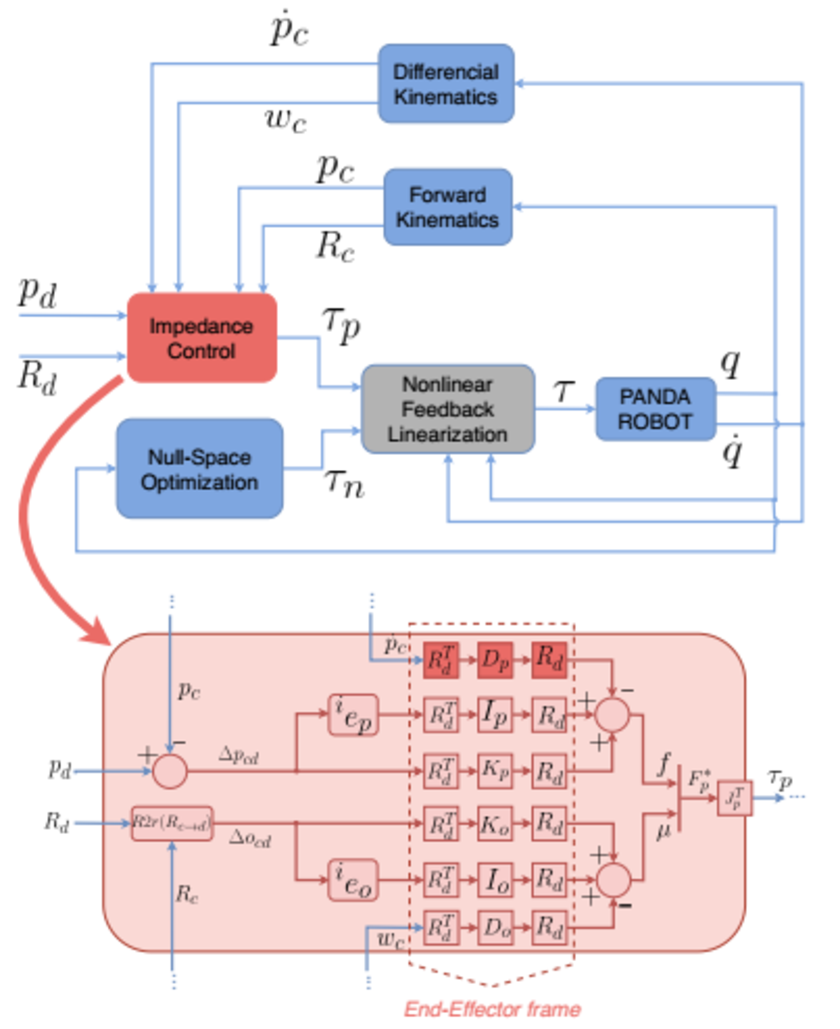
\includegraphics[width=.8\textwidth]{control_architecture_diagram}
	\caption{Control architecture diagram. A Cartesian impedance controller with posture optimisation, where Cartesian positioning is the primary task and posture optimisation is performed in the null-space. \cite{Ochoa2019_control_architecture_robotic_polishing}}
	\label{fig:control_architecture_diagram}
\end{figure}

% subsection control_architectures_cartesian_impedance_posture_optimisation_architecture

% section control_architectures_cartesian_impedance_posture_optimisation

\section{Gravity Compensation Controller}
\label{sec:control_architectures_gravity_compensation}

During co-manipulation, when the operator manually moves the robotic arm, a different control architecture must be used.

In this particular case, a simplified approach was followed. Since the goal is for the operator to freely move the robot end-effector in space, it is important for the manipulation to be as easy as possible. The approach followed was to use the robot in gravity compensation. This means that the robot holds its position when left alone and presents no resistance when pushed/pulled.

The commanded torque $\boldsymbol{\tau}_c$ for this case is

\begin{equation}
    \boldsymbol{\tau}_c = \boldsymbol{g}(\boldsymbol{q}).
\end{equation}

% section control_architectures_gravity_compensation